\documentclass[12pt, fleqn, xcolor=x11names, xcolor=table, aspectratio=169]{beamer}
% \documentclass[xcolor=table]{beamer}
\beamertemplatenavigationsymbolsempty
\usecolortheme{beaver}
\setbeamertemplate{blocks}[rounded=true, shadow=true]
\setbeamertemplate{footline}[page number]
\setbeamercolor{itemize item}{fg=red}
\setbeamercolor{enumerate item}{fg=red}
% \usepackage{jmlda}

%
\usepackage[utf8]{inputenc}
\usepackage[english,russian]{babel}
\usepackage{amssymb,amsfonts,amsmath,mathtext}
\usepackage{subfig}
\usepackage[all]{xy} % xy package for diagrams
\usepackage{array}

\usepackage{multirow}
\usepackage{multicol}% many columns in slide
\usepackage{hyperref}% urls
\usepackage{hhline}%tables
% Your figures are here:
% \usepackage{graphicx}
% \usepackage{epstopdf}
\usepackage{epsfig}
\graphicspath{ {fig/} {../fig/} }

\usepackage{xcolor, color, colortbl}
\usepackage[table]{xcolor}
\definecolor{aquamarine}{rgb}{0.5, 1.0, 0.83}
\definecolor{blue-green}{rgb}{0.0, 0.87, 0.87}
\usepackage{tabularx}
\newcommand\setrow[1]{\gdef\rowmac{#1}#1\ignorespaces}


\newcommand{\diag}{\mathop{\mathrm{diag}}}

%----------------------------------------------------------------------------------------------------------
\title{Оптимизация критерия заданного нейросетевой моделью в задаче детоксификации текста}
\author[А.\,A.~Пилькевич]{А.\,A.~Пилькевич}
\institute{Московский физико-технический институт}
\date{\footnotesize
% \par\smallskip\emph{Курс:} Автоматизация научных исследований\par (практика, В.\,В.~Стрижов)/Группа 874
% \par\smallskip\emph{Эксперт:} В.\,В.~Стрижов
\par\smallskip\emph{Консультант:} А.\,С.~Попов
\par\bigskip\small 2022}
%----------------------------------------------------------------------------------------------------------
\def\vec#1{\mathchoice{\mbox{\boldmath$\displaystyle#1$}}
{\mbox{\boldmath$\textstyle#1$}} {\mbox{\boldmath$\scriptstyle#1$}} {\mbox{\boldmath$\scriptscriptstyle#1$}}}
\begin{document}
%----------------------------------------------------------------------------------------------------------
\begin{frame}
\thispagestyle{empty}
\maketitle
\end{frame}

%-----------------------------------------------------------------------------------------------------
\begin{frame}{\textbf{TODO:} Новизна}
В NLP есть тысячи задач. 
Под каждую задачу скорее всего есть отдельная модель, которая её решила.  
Сейчас большинство SOTA моделей очень дорого переобучать или вообще не возможно.

При этом существуют задачи, качество решения которых оценивают при помощи таких SOTA моделей.
Например: 
качество сгенерированных текстов (смысл, связность, орфография), схожесть исходного и нового текста (перефразировка) и так далее. 

И возникает естественное желание использовать эти модели в качестве функции потерь. 
Но есть одно НО...

\end{frame}


%-----------------------------------------------------------------------------------------------------
\begin{frame}{Детоксификация предложений}

% Преобразуются токсичные предложения с целью сохранения смысла и избавления от токсичных слов или их замене на нейтральный аналог. 

\begin{alertblock}{Задача}
Детоксификация токсичных входных предложений к нейтральному варианту.
\end{alertblock}

\begin{alertblock}{Проблема}
Для оценки качества детоксификации используется \textbf{нейросетевая модель} оценки токсичности.
Но эту модель нельзя использовать в качестве функции потерь из-за отличного токенайзера, так как \textbf{теряется дифференцируемость}. 
\end{alertblock}

\begin{alertblock}{Решение}
В данной работе предлагается переобучать эмбеддинг слой лосс-модели, который будет принимать логиты модели детоксификатора. 
\end{alertblock}

\end{frame}
%-----------------------------------------------------------------------------------------------------
\begin{frame}{Данные и оценка качества}
Задано множество пар:  $\{T_i, D_{i}\}_{i=1}^{N}$, где $T_i$~--- токсичное предложение, $D_{i}$~--- нейтральная версия.  \\

\textit{Пример:} 
\begin{align*}
T_i &= \textit{'Её муженька козла на кол надо посадить'}, \\
D_{i} &=  \textit{'Её мужа нужно наказать'}.
\end{align*}
\textbf{Требуется:} по токсичному предложению построить его нейтральный вариант. 

\textbf{Метрики:}
    \begin{itemize}
        \item Style Transfer Accuracy (STA)~--- выход предобученного Conversational RuBERT дообученного на задачу определения токсичности,
        \item chrF~--- F-мера на основе символьных $n$-грамм.\footnote{chrF: character n-gram F-score for automatic MT evaluation (Popović, 2015)}
    \end{itemize}

\end{frame}

%-----------------------------------------------------------------------------------------------------
\begin{frame}{STA, chrF}

\begin{alertblock}{STA}
Вероятность токсичности предложения. (?)
\end{alertblock}

\begin{alertblock}{chrF}
chrP --- доля символьных n-грамм из предлагаемого предложения, которые имеются в оригинальном. \\
chrR --- доля символьных n-грамм из оригинального предложения, которые представлены в предлагаемом.  \\ 
Тогда финальная формула:
\begin{gather*}
    \text{chrF}\beta = (1 + \beta^2) \frac{\text{chrP} \cdot \text{chrR}}{\beta^2 \text{chrP} + \text{chrR}},
\end{gather*}
где chrP, chrR считаются как среднее по всем предложениям. 
\end{alertblock}

\end{frame}

%----------------------------------------------------------------------------------------------------------

\begin{frame}{Baseline и первые шаги}
Берётся предобученный русскоязычный трансформер T5\footnote{\url{https://huggingface.co/sberbank-ai/ruT5-base}} (\textit{детоксификатор}).
Он дообучается на задаче seq-to-seq для пар $x, y \in \{T_i, D_{i}\}_{i=1}^{N}$:
\begin{gather*}
    Loss(p^*, p) = -\sum_{t=1}^{n} \sum_{v=1}^{|V|} p^{*}_{t, v} \log p_{t, v} = -\sum_{t=1}^{n} \log \left(p(y_{t} | y_{<t}, x) \right),
\end{gather*}
где $p^{*}$--- истинная вероятность, $p$~--- предсказанная.

\begin{alertblock}{Предложение и проблемы}
Хотим использовать \textbf{STA в качестве функции потерь}. 
Это позволит учитывать токсичность получаемых предложений и корректировать их.
% Оптимизация детоксификатора на основе STA явно решает задачу детоксификации.

Но в данном случае нет дифференцируемости, так как \textbf{нет отображения между токенами различных токенайзеров}. 
\end{alertblock}

\end{frame}

% %----------------------------------------------------------------------------------------------------------

% \begin{frame}{Адаптер}

% Будем использовать вместо эмбеддингов лосс-модели адаптер, который принимает на вход логиты детоксификатора и приближает истинные эмбеддинги. 

% \begin{figure}[ht]
%     {\includegraphics[width=1.\textwidth]{images/adapter.pdf}}
% \end{figure}

% \end{frame}

%----------------------------------------------------------------------------------------------------------

\begin{frame}{Адаптер}

Вместо эмбеддингов STA-модели используется адаптер, который принимает на вход логиты детоксификатора и приближает истинные эмбеддинги. 

\vfill

\begin{columns}
\column{.7\textwidth}
\textbf{Выход STA-модели}: $ p_i$~--- вероятность токсичности предложения $D_{i}$.

\textbf{Функция потерь адаптера}: $KL(p_i, p_i^{*})$, где $p_i^{*}$~--- вероятность, полученная с использованием адаптера.

\begin{alertblock}{Алгоритм обучения}
\begin{enumerate}
    \item Дообучается T5 на задаче seq-to-seq.
    \item Обучаем адаптер при фиксированных весах детоксификатора и STA-модели.
\end{enumerate}
\end{alertblock}

\column{.3\textwidth}
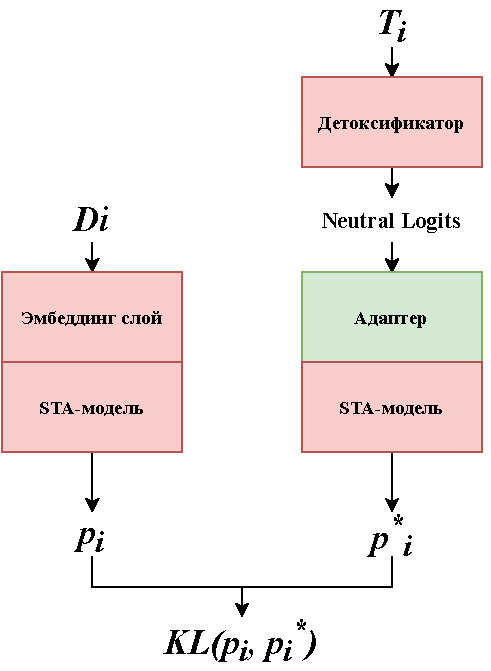
\includegraphics[width=3.5cm]{images/adapter_train.drawio.pdf}
\end{columns} 
\end{frame}

%----------------------------------------------------------------------------------------------------------

\begin{frame}{Дообучение детоксификатора}
При дообучении детоксификатора используется схожая идея с обучением порождающих моделей при использовании adversarial loss\footnote{Goodfellow, I. et al., 2014. Generative adversarial nets. In Advances in neural information processing systems. pp. 2672–2680.}.

Пусть $CE, TP$~--- значение кросс-энтропии и выход STA-модели (вероятность токсичности) на батче.
И пусть $f(*, *)$~--- произвольная функция, такая что $f: \mathbb{R}^2 \to \mathbb{R}$.
Тогда

\begin{alertblock}{Алгоритм\footnote{В обоих случаях веса STA-модели фиксированы, как и везде до этого}}
\begin{enumerate}
    \item $N$ батчей обучается детоксификатор на $f(\text{CE, TP})$, при фиксированном адаптаре. 
    \item $M$ батчей обучается адаптер на KL-divergence, при фиксированном детоксификаторе.
\end{enumerate}
\end{alertblock}
\end{frame}

%----------------------------------------------------------------------------------------------------------

\begin{frame}{Эксперименты и результаты}

Размер обучающего датасета: $N = 11136$ пар $\left(T_i, D_i \right)$, $10\%$ использовались для валидации во время обучения.
Размер тестового датасета: $N_t = 800$ предложений.

В качестве $f(\text{CE, TP})$ брались следующие комбинации: 
\begin{align*}
    f(\text{CE, TP}) &= \text{CE} \cdot \text{TP}, \\
    f(\text{CE, TP}) &= w_1 \text{CE} + w_2 \text{TP}.
\end{align*}

Результаты экспериментов в различных сетапах обучения:

\begin{table}[ht]
\centering
 \begin{tabular}{|c|c c c|} 
 \hline
 Эксперимент & STA & chrF1 & STA*chrF1 \\ [0.5ex] 
 \hline
 CE only & 0.739 & 0.578 & 0.427 \\ 
 \rowcolor{aquamarine} GAN style, $\text{CE} + 10 \cdot \text{TP}$ & 0.813 & 0.569 & 0.462 \\
  GAN style, $\text{CE} \cdot \text{TP}$  & 0.754 & 0.574 & 0.439 \\
 Model loss only & 0.998 & 0.119 & 0.119 \\ 
 \hline
 \end{tabular}
\end{table}

\end{frame}

%----------------------------------------------------------------------------------------------------------

\begin{frame}{Эксперименты и результаты}

Подбор способа обучения и проверка стат. значимости:\footnote{При запусках экспериментов использовались различные seed}
\begin{table}[ht]
\centering
 \begin{tabular}{|c|c c c|} 
 \hline
 Эксперимент & STA & chrF1 & STA*chrF1 \\ [0.5ex] 
 \hline
 CE only & $0.744 \pm 0.010$ & $0.575 \pm 0.002$ & $0.430 \pm 0.042$ \\ 
 Same batch\footnote{На одном батче сперва оптимизировался детоксификатор, затем адаптер}, $\text{CE} \cdot \text{TP}$ & $0.776 \pm 0.015$ & $0.569 \pm 0.004$ & $0.442 \pm 0.006$ \\
 Same batch, $\text{CE} + 10 \cdot \text{TP}$ & $0.774 \pm 0.011$ & $0.561 \pm 0.012$ & $0.435 \pm 0.013$ \\

  \hline
 \end{tabular}
\end{table}

\textbf{TODO:} Эксперимент с одновременным обучением адаптера и модели

Обучение адаптера на эмбеддингах детоксификатора вместо логитов. 
\begin{table}[ht]
\centering
 \begin{tabular}{|c|c c c|} 
 \hline
 Эксперимент & STA & chrF1 & STA*chrF1 \\ [0.5ex] 
 \hline
 CE only & 0.742 & 0.577 & 0.428  \\ 
 Adapter on embs, & 0.639 & 0.544 & 0.348 \\

  \hline
 \end{tabular}
\end{table}

\end{frame}


%----------------------------------------------------------------------------------------------------------
\begin{frame}{Заключение}
    \begin{enumerate}
        \item Предложен алгоритм использования модели в качестве функции потерь в условиях отсутствия дифференцируемость из-за различных токенайзеров.
        
        \item Продемонстрирована работоспособность и эффективность предложенного метода.  
        
        \item Подобраны оптимальный параметры обучения. 
    \end{enumerate}
\end{frame}

%----------------------------------------------------------------------------------------------------------
\end{document} 
